\documentclass[../tfg.tex]{subfiles}

\begin{document}

\section{ret2libc}

In a traditional stack overflow we try to return to some shellcode in a buffer we can control. For this reason, a countermeasure appeared to prevent execution on writable segments (see \ref{stack_overflow_countermeasures:NX}). With this limitation, we cannot inject code anymore. The solution comes from reusing the existing code to achieve our goals, like in the \textbf{ret2win} example (see \ref{stack_overflow:ret2win}). Libc is a library loaded on almost all processes, so returning to a function inside libc is always an option. Furthermore, libc declares \texttt{system}, a very well suited win function.\\

To perform the call to \texttt{system} we need to prepare the stack with the parameters that the compiler would set for a compiled call to \texttt{system}:
\begin{lstlisting}
int system(const char* command);
\end{lstlisting}
We require the address of \texttt{command} to be present on the stack, before (higher addresses) the overwritten return address.

\begin{figure}[H]
    \centering
    \subfile{../imgs/rop/ret2libc_stack_layout}
    \caption{ret2libc stack layout}
    \label{fig:ret2libc_stack_layout}
\end{figure}

\subsection*{Example}
For this example we will use a custom vulnerable 32bit program compiled with all the protections disabled, with no debugging symbols and ASLR turned off for the operating system.

\lstinputlisting[language=C, caption={example.c}]{../../src/rop/main.c}

Using our layout for a ret2libc exploit we need to plug in the addresses of the \texttt{system} function and a \texttt{"/bin/sh"} string. Because the binary was compiled with no debugging symbols we can't search for the symbol inside \texttt{gdb} or another debugger. But because ASLR is disabled, we know where libc will be loaded. We could get the offset of \texttt{system} from the libc base address to know where it will be located at runtime.

\begin{figure}[H]
    \centering
    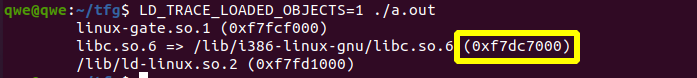
\includegraphics[width=\linewidth]{imgs/rop/ret2libc_libc_base.png}
    \caption{libc base address}
    \label{fig:ret2libc_libc_base}
\end{figure}

\begin{figure}[H]
    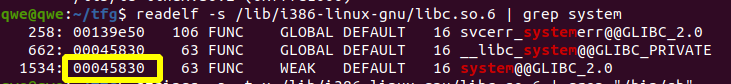
\includegraphics[width=\linewidth]{imgs/rop/ret2libc_libc_system.png}
    \caption{\texttt{system} offset from libc base address}
    \label{fig:ret2libc_libc_system}
\end{figure}

\begin{figure}[H]
    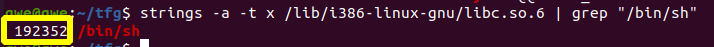
\includegraphics[width=\linewidth]{imgs/rop/ret2libc_libc_binsh.png}
    \caption{\texttt{"/bin/sh"} string offset from libc base address}
    \label{fig:ret2libc_libc_binsh}
\end{figure}

Knowing all those addresses we can plug them into a python script taking into account how the stack will unwind and what \texttt{system} expects to be on the stack.

\lstinputlisting[language=python, caption={exploit.py}]{../../src/rop/exploit.py}

Once we crafted the exploit we need to concatenate it with \texttt{stdin} to obtain access to the shell (see \ref{stack_overflows:shell_concatenate_stdin}).

\begin{figure}[H]
    \centering
    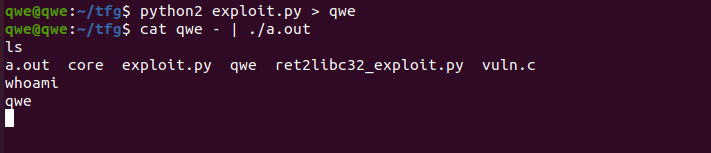
\includegraphics[width=\linewidth]{imgs/rop/ret2libc_exploit.png}
    \caption{ret2libc exploit}
    \label{fig:ret2libc_exploit}
\end{figure}

When compiling a binary for 64bits, the default calling convention used by \texttt{gcc} in Linux systems is the \emph{System V AMD64 ABI}, which specifies that the first 6 parameters (integers or pointers) are passed in registers instead of being pushed on the stack. That represents a problem for our ret2libc technique, as we only control the stack.

To overcome this issue we will use return-oriented programming, the generalized and refined form of a ret2anything exploit.

\section{ROP}
Return-oriented programming is a programming paradigm by which an \textbf{attacker can induce arbitrary behavior} in a program \textbf{without code injection}. This defeats the countermeasure of NX/DEP/W$\oplus$X.

This technique presents a whole new programming paradigm (an esoteric one): using the code of a existing program to create another program inside the process, by means of concatenating return addresses and a stack overflow.

In a typical stack overflow, we override the return stack writing only one address.

\subsection{ROP Gadgets}
ROP Gadgets are machine code snippets that end with a \texttt{ret} instruction. We can chain them together by pushing their start addresses in sequence on a stack overflow attack, creating a \textbf{ROP chain}.

\begin{figure}[H]
    \centering
    \subfile{../imgs/rop/rop_chain}
    \caption{ROP chain}
    \label{fig:rop_chain}
\end{figure}

\subsection*{Example}
We will use the same program for the ret2libc example, but compiled for 64bit. Because of the default calling convention for 64bit gcc binaries on Linux, we need to pass the \texttt{"/bin/sh"} string pointer in the register \texttt{rdi}. To accomplish this, we will search for gadgets on the binary.

Because we control the stack thanks to the stack overflow, we could use a \texttt{pop rdi} instruction to put our pointer into the register.

\begin{figure}[H]
    \centering
    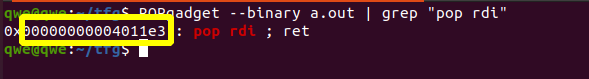
\includegraphics[width=\linewidth]{imgs/rop/rop_gadget.png}
    \caption{ROP gadget \texttt{pop rdi; ret}}
    \label{fig:rop_gadget}
\end{figure}

%https://stackoverflow.com/questions/60729616/segfault-in-ret2libc-attack-but-not-hardcoded-system-call
In this case we also need a NOP gadget to achieve stack alignment. This gadget does nothing more than calling the following gadget on the chain and with this addition our whole rop chain is 32 bytes long, which is aligned for the 16 byte stack. If this gadget was omitted, the rop chain would be 24 bytes long, which is not divisible by 16 and therefore, would not be aligned.

\begin{figure}[H]
    \centering
    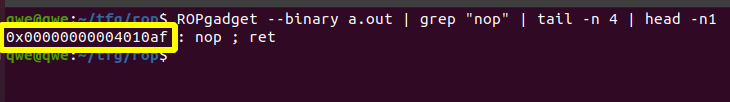
\includegraphics[width=\linewidth]{imgs/rop/rop_nop_gadget.png}
    \caption{NOP gadget}
    \label{fig:rop_nop_gadget}
\end{figure}

Before calling \texttt{system} we have to set up the string pointer in \texttt{rdi}, so this gadget will be the first we will return to, followed by the address of \texttt{"/bin/sh"} and the address of \texttt{system}.

\begin{figure}[H]
    \centering
    \subfile{../imgs/rop/example_rop_chain}
    \caption{Stack layout for example}
    \label{fig:rop_stack_layout_example}
\end{figure}

We collect again the addresses of interest because we are now using the 64bit libc.

\begin{figure}[H]
    \centering
    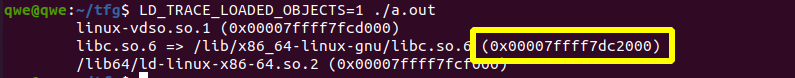
\includegraphics[width=\linewidth]{imgs/rop/rop_libc_base.png}
    \caption{libc base address at runtime}
\end{figure}

\begin{figure}[H]
    \centering
    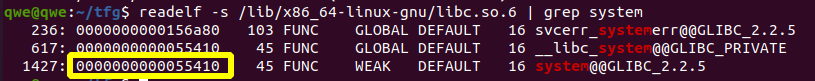
\includegraphics[width=\linewidth]{imgs/rop/rop_libc_system.png}
    \caption{\texttt{system} offset from libc base address}
\end{figure}

\begin{figure}[H]
    \centering
    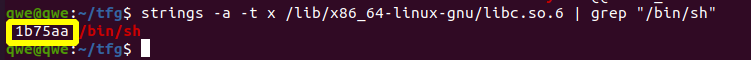
\includegraphics[width=\linewidth]{imgs/rop/rop_libc_binsh.png}
    \caption{\texttt{"/bin/sh"} offset from libc base address}
\end{figure}

\lstinputlisting[language=python, caption={exploit64.py}]{../../src/rop/exploit64.py}

Again, to keep the shell open we need to concatenate the exploit with \texttt{stdin}.

\begin{figure}[H]
    \centering
    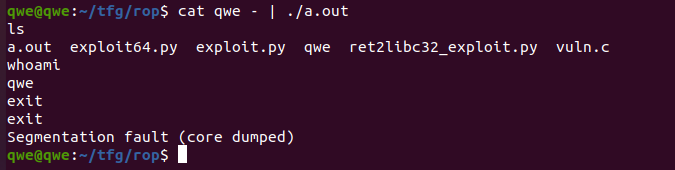
\includegraphics[width=\linewidth]{imgs/rop/rop_shell.png}
    \caption{Successful exploitation of the rop chain}
\end{figure}

\section{Stack pivoting}
A stack pivot attack consist of creating a fake stack somewhere in memory and tricking the program to use it as its stack. This technique is useful when the legitimate stack lacks space for a ROP chain.

For this attack it is necessary to control the stack pointer register to be able to change the stack of the program for the attacker controlled one. To accomplish this, we need to find some gadgets:

\begin{enumerate}
    \item \texttt{pop rsp}. Ideal gadget in theory. Hardly found in any executable.
    \item \texttt{xchg reg, rsp}. Used in combination with \texttt{pop reg} to write a value on \texttt{reg} to later exchange it with \texttt{rsp}. Requires 16 bytes of stack space after the return address.
    \item \texttt{leave; ret}. All functions except \texttt{main} are ended with \texttt{leave; ret}. That makes this case the most plausible. The \texttt{leave} instruction is equivalent to:
        \begin{lstlisting}
            mov rsp, rbp
            pop rbp
        \end{lstlisting}
        If we call \texttt{leave} two consecutive times, the first \texttt{pop rbp} will be used to set \texttt{rsp} on the second \texttt{leave}.
        \begin{figure}[H]
            \centering
            \subfile{../imgs/rop/stack_pivot_stack.tex}
            \caption{Stack layout for a stack pivoting attack}
        \end{figure}
        %% TODO: use this case for arbitrary read, if a function uses [rbp+0x10] for reading function arguments, rbp can be set to leak info, like stack canaries
\end{enumerate}

\subsection*{Example}
In this exercise the objective is to pivot the stack to \texttt{buffer}. I will use the \texttt{leave} gadget to trigger the pivot.

First, we need the \texttt{leave} gadget.
\begin{figure}[H]
    \centering
    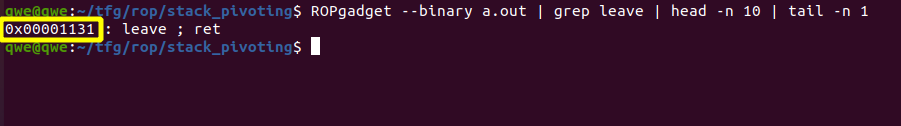
\includegraphics[width=\linewidth]{imgs/rop/stack_pivoting/leave_gadget.png}
    \caption{\texttt{leave} gadget}
    \label{fig:stack_pivoting_leave_gadget}
\end{figure}

The address shown in Figure \ref{fig:stack_pivoting_leave_gadget} is only an offset from the base address of the binary. To make it usable add it to the base address.


Once we pivoted the stack, on the \texttt{leave} gadget, the following \texttt{ret} instruction will pop from \texttt{buffer} the return address. In this case, I filled it with the address of \texttt{win} so at the end, we will jump to that function.

\lstinputlisting[language={python}]{../../src/rop/stack_pivoting/exploit.py}

With this exploit, the sequence of instructions we want to execute is the following.
\begin{figure}[H]
    \centering
    \subfile{../imgs/rop/stack_pivoting/instr_sequence.tex}
    \caption{Stack pivoting example: instruction sequence}
\end{figure}

Setting a breakpoint on \texttt{win} we can see that now, the \texttt{esp} register points to the user supplied buffer. We have pivoted the stack.

\begin{figure}[H]
    \centering
    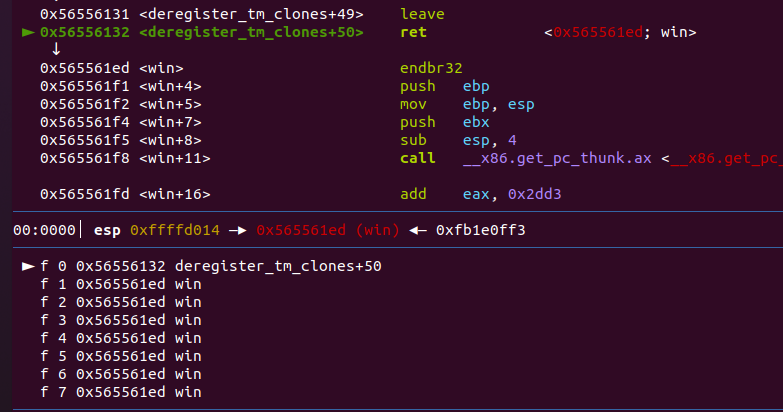
\includegraphics[width=\linewidth]{imgs/rop/stack_pivoting/esp_points_to_buffer.png}
    \caption{\texttt{esp} points to \texttt{buffer}}
\end{figure}

\begin{figure}[H]
    \centering
    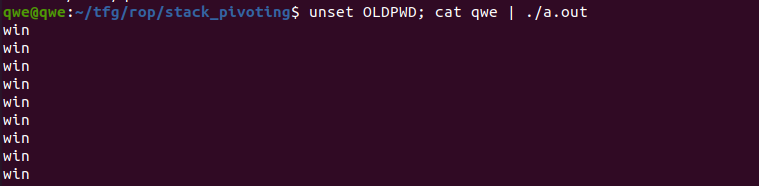
\includegraphics[width=\linewidth]{imgs/rop/stack_pivoting/success1.png}
    \caption{Succesful exploitation}
\end{figure}

\section{ret2dlresolve}
Technique for executing dynamically linked functions without knowledge of their addresses. The attacker tricks the binary into resolving a function of its choice into the Procedure Linkage Table, bypassing ASLR.

When the binary calls a dynamically linked function for the first time and has \emph{lazy binding} enabled (no RELRO or Partial RELRO), it is going to jump into the PLT section to try to resolve the symbol on demand.

\subsection{Structures}
In order to resolve a symbol, 3 structures are needed. By faking them, we could trick the loader to resolve a symbol of our choice.

\begin{minipage}[c]{0.45\linewidth}
\subsubsection{JMPREL}
Corresponds to the \texttt{rel.plt} segment and holds the \textbf{relocation table}. This table maps a symbol to an offset on the GOT. The \texttt{r\_info} field gives us the index  of the symbol on the SYMTAB.

\subsubsection{SYMTAB}
Symbol table. Stores information about the symbols. The most important field for this exploit is \texttt{st\_name} which is the offset on the STRTAB structure.

\subsubsection{STRTAB}
String table. Stores the name of the symbols.
\end{minipage}
\begin{minipage}[c]{0.45\linewidth}
\begin{figure}[H]
    \centering
    \subfile{../imgs/rop/ret2dlresolve_structures.tex}
\end{figure}
\end{minipage}

\subsection{Symbol resolution}
When linking, the linker is going to replace every dynamic call to an entry on the PLT table, located on the \texttt{.plt} table. The PLT table contains executable code formed by stubs. This stubs will jump to the GOT table to try to execute the intended function if it is resolved but if the function is not present on the GOT table (the function has not been resolved yet) the GOT code will return to the PLT entry to call the resolver.

The process for calling a dynamic function is the following:

\begin{enumerate}
    \item Control is transferred to the \texttt{.plt} entry of the function, for example \texttt{puts@plt}.
    \item That \texttt{.plt} entry gets a value from the \texttt{.got} section. This value can have two different interpretations:
    \begin{enumerate}
            \item If the symbol has been previously resolved, the value points to where the function has been loaded at runtime.
            \begin{enumerate}
                \item Control is transferred to the resolved function, for example \texttt{puts@libc}.
            \end{enumerate}
        \item If the symbol has not been previously resolved, the value points back to a different part of the symbol entry on the \texttt{.plt}.%to the default entry on the \texttt{.plt} section.
            \begin{enumerate}
                \item Push the \texttt{reloc\_index}. This argument is the entry index on the \texttt{JMPREL} table.
                \item Jump to the default entry stub on the \texttt{.plt}.
                \begin{enumerate}
                    \item Push the \texttt{link\_map} into the stack.
                    \item Call \texttt{\_\_dl\_runtime\_resolve}.
                \end{enumerate}
                \item Call the resolved symbol.
            \end{enumerate}
    \end{enumerate}
\end{enumerate}

Every time a symbol is resolved via \texttt{\_\_dl\_runtime\_resolve}, the corresponding GOT entry is updated to point to the resolved address.

\begin{figure}[H]
    \centering
    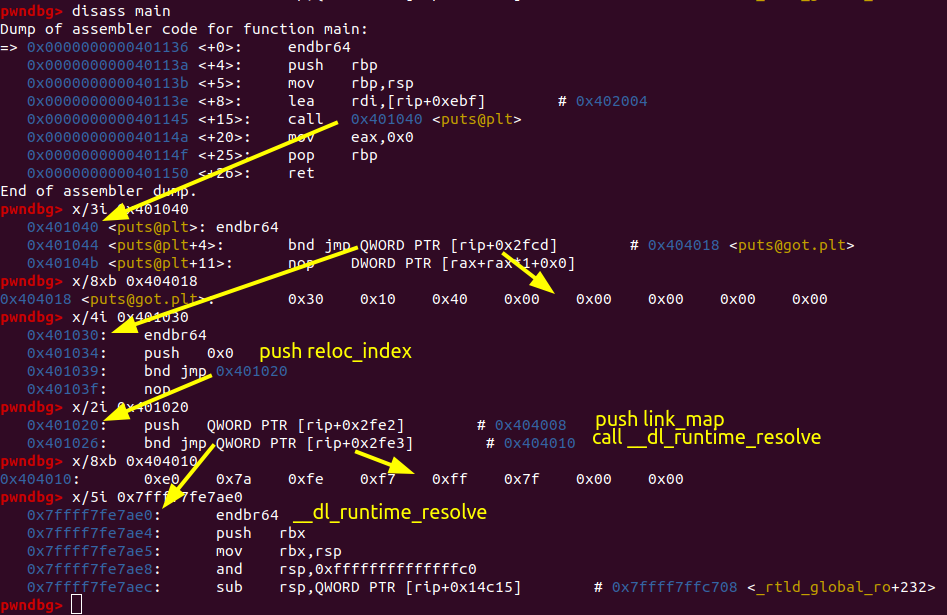
\includegraphics[width=\linewidth]{imgs/rop/ret2dlresolve/plt_got_dlresolve.png}
    \caption{\texttt{\_\_dl\_runtime\_resolve} execution path}
    \label{fig:dl_resolve_exec_path}
    %\subfile{../imgs/rop/ret2dlresolve/plt_got_call.tex}
\end{figure}

\texttt{\_\_dl\_runtime\_resolve} receives as parameters the \texttt{link\_map} and the \texttt{reloc\_index} \textbf{in the stack}, even for x86\_64 systems. Then it will move this parameters into \texttt{rsi} and \texttt{rdi} respectively and call \texttt{\_dl\_fixup}, which is the resolver.

The \href{https://elixir.bootlin.com/glibc/latest/source/sysdeps/x86_64/dl-trampoline.h#L60}{source code for the \texttt{\_\_dl\_runtime\_resolve}} function can be found on the glibc source code.

Faking the data structures and passing them to \texttt{\_\_dl\_runtime\_resolve()} effectively corrupts the GOT table and hijacks function calls.

\texttt{\_\_dl\_runtime\_resolve} is in reality only a wrapper for \texttt{\_dl\_fixup}, which in turns does all the heavy lifting for the symbol resolution. Here we can find all the computations needed to link the JMPREL, SYMTAB and STRTAB structures together to get the symbol information.

\begin{lstlisting}[caption={\texttt{\_dl\_fixup} pseudocode.}]
#define ELF64_R_SYM ((i) >> 32)

void* _dl_fixup(struct link_map* l, Elf64_Word reloc_arg) {
    Elf64_Rela* reloc_entry = JMPREL + (reloc_arg * sizeof(Elf64_Rela));
    Elf64_Sym* = symbol_entry = SYMTAB[ELF64_R_SYM(reloc_entry->r_info)];
    const char* symbol_string = STRTAB + symbol_entry->st_name;
    /* ... */
}
\end{lstlisting}

\subsection*{Example}
Now we can use a buffer overflow to trick \texttt{\_\_dl\_runtime\_resolve} into resolving the symbols of our choosing. To do that, we need to jump to the start of the \texttt{.plt} section, where the code for pushing the \texttt{link\_list} and calling \texttt{\_\_dl\_runtime\_resolve} is found. Before the jump we need to set on the top of the stack the index on the JMPREL that we want to resolve. This index will have to point to our fake data structures, written on some buffer, attending the previous formula.

\begin{lstlisting}
Elf64_Rela* reloc_entry = JMPREL + (reloc_arg * sizeof(Elf64_Rela));
\end{lstlisting}

The address of JMPREL can be found by examining the ELF headers of the executable. If the binary has PIE enabled, the value will be an offset from the image base; if PIE is not enabled, the value is an absolute address.

\begin{lstlisting}
readelf -d a.out | grep -e JMPREL -e STRTAB -e SYMTAB
\end{lstlisting}

\begin{figure}[H]
    \centering
    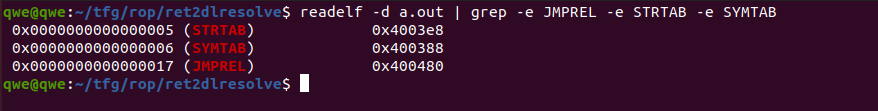
\includegraphics[width=\linewidth]{imgs/rop/ret2dlresolve/tables.png}
    \caption{Addresses of the most important tables for the exploit}
\end{figure}

\texttt{reloc\_arg} has as type \texttt{Elf64\_Word}, an alias for a 32bit unsigned integer. That imposes a restriction: The distance between the JMPREL and our fake data cannot be greater than $\texttt{0xffffffff} \times \texttt{sizeof(Elf64\_Rela)} = \texttt{0x17FFFFFFE8}$. Often we only can write to the stack, which is usually too far away from the JMPREL. In order to be in range, we will need to call a \texttt{read} into a more proper location. This exploit is going to have 2 stages:

\begin{enumerate}
    \item ROP chain to write our fake data structures in another buffer near JMPREL, SYMTAB and STRTAB.
    \item Jump to \texttt{\_\_dl\_runtime\_resolve} with \texttt{reloc\_arg} pointing into the fake data structures.
\end{enumerate}

\subsubsection{Stage 1}
A simple ROP chain to call \texttt{read} on a convenient address that will write the fake data structures to feed them to the resolver.
\lstinputlisting[language=python, linerange={20-31}, firstnumber=20]{../../src/rop/ret2dlresolve/exploit.py}

 The section where the buffer for the fake data will be written must have RW permissions and must be mapped after the tables. To find such a section we can search on the ELF section headers.

\begin{figure}[H]
    \centering
    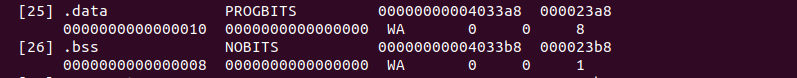
\includegraphics[width=\linewidth]{imgs/rop/ret2dlresolve/data_segments.png}
    \caption{\texttt{.data} and \texttt{.bss} segments of the process}
\end{figure}

\begin{figure}[H]
    \centering
    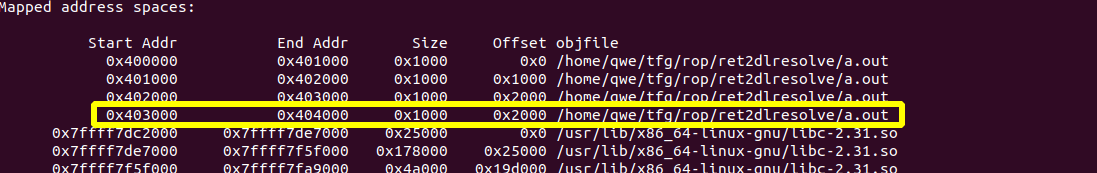
\includegraphics[width=\linewidth]{imgs/rop/ret2dlresolve/mappings.png}
    \caption{Mapped segments of the process}
\end{figure}
I will use the last portion of the last segment of \texttt{a.out}, the address \texttt{0x403e00}. Because of
$$ (\texttt{0x403e00} - \texttt{0x400480})\ \mathrm{mod}\ \texttt{0x18} \equiv 8 $$
the first two bytes of the second buffer will be padding for the relocation entry, that is going to start at \texttt{0x403e10}, which is divisible by 24.
Now we compute the value that \texttt{\_\_dl\_resolve\_runtime} requires to find the symbol.
$$ \frac{(\texttt{0x403e10} - \texttt{0x400480})}{\texttt{0x18}} = \texttt{0x266} $$
That will be the relocation index passed as a parameter to the resolver.

\begin{figure}[H]
    \centering
    \subfile{../imgs/rop/ret2dlresolve/offsets.tex}
    \caption{Offsets from the tables to the second buffer}
\end{figure}

\subsubsection{Stage 2}
Now we fill the entries in sequence. For the relocation entry, the important field is \texttt{r\_info}. In x86\_64 Linux systems, 32 highest bits of this field hold the offset from the SYMTAB to the symbol entry. The lowest 32 bits stores the type of relocation. To bypass a \href{https://elixir.bootlin.com/glibc/glibc-2.33/source/elf/dl-runtime.c#L76}{check} in \texttt{\_dl\_fixup} these bits must be set to 7. The \texttt{Elf64\_Rela} struct has one more field of 64 bits but since this field is unused, I overlapped it with the symbol entry. This trick also helps me with padding as \texttt{0x403e18} is not aligned with SYMTAB.
The computation for the index of the symbol entry follows the same scheme that the relocation offset.

\lstinputlisting[language=python, linerange={42-48}, firstnumber=42]{../../src/rop/ret2dlresolve/exploit.py}

The symbol entry has been zeroed out except for the \texttt{st\_name} field which stores the distance in bytes from STRTAB to a string

\lstinputlisting[language=python, linerange={49-58}, firstnumber=49]{../../src/rop/ret2dlresolve/exploit.py}

Now, going back to the ROP chain, we need to invoke \texttt{\_\_dl\_runtime\_resolve} emulating a legitimate call. To do this, before calling the resolver we need to set up the arguments for \texttt{system} as it is was already resolved and we were calling it directly: with \texttt{rdi} pointing to \texttt{"/bin/sh"}.
Chaining a \texttt{pop rdi; ret} gadget followed by the address of the \texttt{"/bin/sh"} string that we put on the second buffer, after the \texttt{system} string. Once the argument is correctly set, the following byte on the ROP chain should be the address of the start of the \texttt{.plt} section, that as shown in \ref{fig:dl_resolve_exec_path} stores a default stub for calling the resolver, pushing the \texttt{link\_map} into the stack and jumping into \texttt{\_\_dl\_runtime\_resolve}.

\lstinputlisting[language=python, linerange={32-38}, firstnumber=32]{../../src/rop/ret2dlresolve/exploit.py}

\begin{figure}[H]
    \centering
    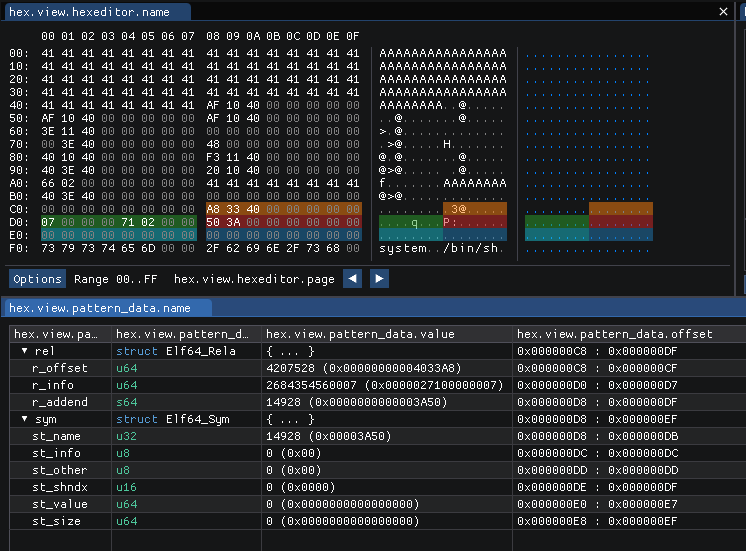
\includegraphics[width=\linewidth]{imgs/rop/ret2dlresolve/dl_payload.png}
    \caption{Bytes of the exploit}
\end{figure}

\begin{figure}[H]
    \centering
    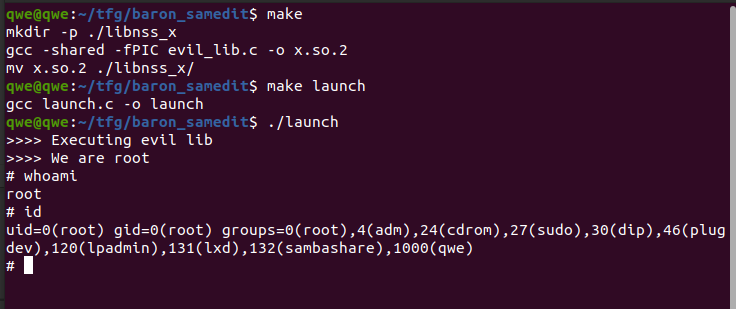
\includegraphics[width=\linewidth]{imgs/rop/ret2dlresolve/success.png}
    \caption{Successful exploitation of an ret2dlresolve attack}
\end{figure}

\section{Sigreturn-oriented programming}
Sigreturn-oriented programming (SROP) exploits the mechanism of handling signals on POSIX systems. These systems implement the \texttt{sigreturn} system call, tasked with restoring the CPU registers with stack values, among other things. By corrupting stack values, an attacker can set the CPU register values at will.

\subsection{Signal handler mechanism}
When a signal is triggered, a context switch is performed. A context switch implies that the state of the current execution must be saved, that is, all the CPU registers are pushed onto the stack along with some additional data. Once the signal has been handled, a \texttt{sigreturn} system call is called and the CPU registers values are restored.

\subsection{\texttt{sigcontext} struct}
When the \texttt{sigreturn} syscall is called, it expects to found a \texttt{sigframe} struct on the top of the stack. The \texttt{sigframe} is a structure that holds several pieces of information for restoring the context of the process. One of these pieces is the \texttt{sigcontext} struct.
The \texttt{sigcontext} struct stores the values of the CPU registers, its flags and the state of the floating point unit. Its definition is dependent on architecture and operating system, but for example, the definition for Linux x86 and x86\_64 systems can be found in the \href{https://elixir.bootlin.com/linux/v5.12.7/source/arch/x86/include/uapi/asm/sigcontext.h#L300}{Linux kernel source}.

\subsection{SROP}
SROP is all about creating a fake signal frame on the stack and call \texttt{sigreturn} to control all the registers on the CPU. First, the call to the syscall is triggered with conventional ROP gadgets. On Linux systems, syscalls are invoked in function of the value of \texttt{rax} when the \texttt{syscall} instruction gets executed. The \texttt{rax} value for the \texttt{sigreturn} syscall is \texttt{0xf} on x86\_64 bit Linux systems and \texttt{0x77} for x86 bit Linux systems.

Once we placed the correct value on \texttt{rax} and executed \texttt{syscall}, \texttt{sigreturn} is going to be executed by the kernel, and it expects a signal frame on the top of the stack. By setting the correct values on the signal frame we can control what we are going to execute next.

\begin{figure}[H]
    \centering
    \subfile{../imgs/rop/srop/srop_layout.tex}
    \caption{Layout of a SROP exploit in Linux x86\_64\cite{srop:paper}}
\end{figure}

\subsection*{Example}
First, we need a simple ROP chain that calls a system call. For that we need a \texttt{pop rax} gadget that sets the correct syscall number on the \texttt{rax} register. Then we execute the \texttt{syscall} instruction with a \texttt{syscall} gadget. The \texttt{sigreturn} syscall has the number \texttt{0xf}.

\begin{figure}[H]
    \centering
    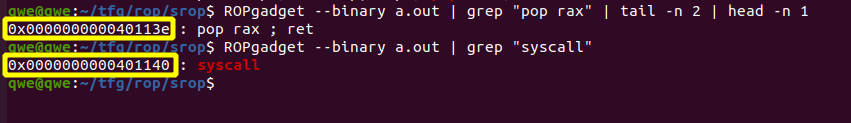
\includegraphics[width=\linewidth]{imgs/rop/srop/srop_gadgets.png}
    \caption{SROP gadgets}
\end{figure}

\lstinputlisting[linerange={15-18}, firstnumber=15]{../../src/rop/srop/exploit.py}

Up to this point this is a normal ROP chain sequence. Now we need to concatenate the \texttt{sigcontext} struct for the \texttt{sigreturn} syscall.

We are going to call \texttt{execve("/bin/sh")} from the signal frame. In order to do that, we need to set the correct registers.
\begin{itemize}
    \item[\texttt{rdi}]: executable file path to run. In our case it is the address of a \texttt{"/bin/sh"} string.
    \item[\texttt{rax}]: \texttt{0x3b}, the \texttt{execve} syscall number.
    \item[\texttt{rsp}]: zeroing this value can be dangerous and cause a segfault. Just point it to some random stack address.
    \item[\texttt{rip}]: because \texttt{execve} is a system call we can reuse the syscall gadget we used previously on the ROP chain.
    \item[\texttt{cs}]: code segment. Used implicitly in the instructions that modify control flow. Necessary to jump around. The value is taken from debugging the program.
    \item[\texttt{ss}]: another segment register. Zeroing it causes segfault. The value is taken from debugging the program.
\end{itemize}
All the other fields are zeroed out.

%\lstinputlisting[linerange={33-46}, firstnumber=33]{../../src/rop/srop/exploit.py}

\begin{figure}[H]
    \centering
    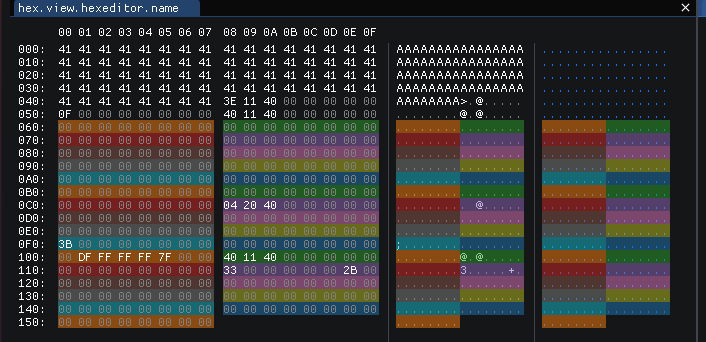
\includegraphics[width=\linewidth]{imgs/rop/srop/srop_bytes.png}
    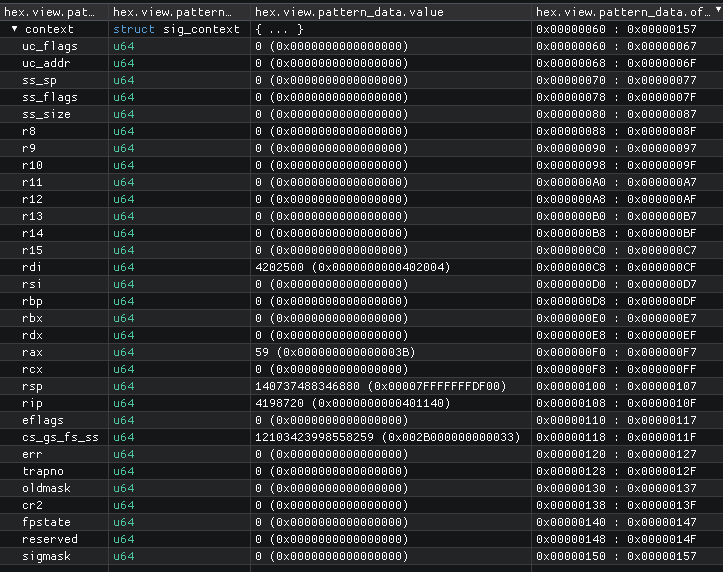
\includegraphics[width=\linewidth]{imgs/rop/srop/srop_struct.png}
    \caption{SROP payload}
\end{figure}

\begin{figure}[H]
    \centering
    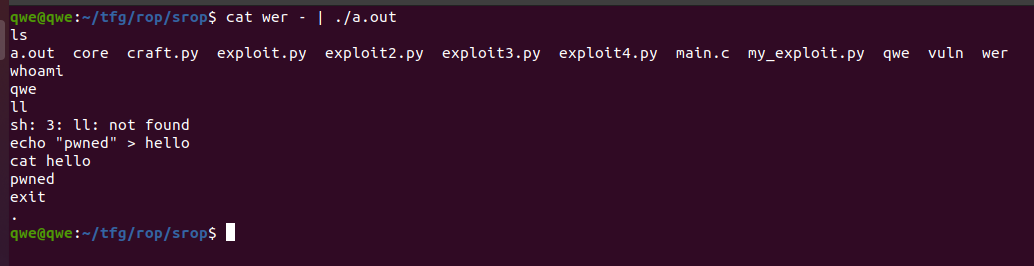
\includegraphics[width=\linewidth]{imgs/rop/srop/srop_success.png}
    \caption{Successful exploitation of an SROP exploit}
\end{figure}

\end{document}

